\documentclass[minted]{protocol}
% Required
\title{Komponentenbasierte Programmierung}
\author{Ebenstein Michael}
% Optional
\mysubtitle{Laborprotokoll}
\mysubject{Systemtechnik Labor}
\mycourse{4HIT 2017/18, Gruppe B}
% Version
\myteacher{Michael Borko}
\myversion{1.1}
\mybegin{5. Juni 2018}
\myfinish{7. Juni 2018}
% \setcode{frame=single} 			% Add a frame to codes (single, lines)
% \setcode{bgcolor=MyLightGray}		% Add a background to codes (minted only)
% \usemintedstyle{rainbow_dash} 	% autumn, rainbow_dash, tango (default), trac

\begin{document}
% \thispagestyle{fancy}				% Makes the first page fancy too
% \begin{abstract}\end{abstract} 	% Add a short overview
\section{Einführung}
Diese Übung zeigt die Anwendung von komponentenbasierter Programmierung mittels Webframeworks.

\subsection{Ziele}

Das Ziel dieser Übung ist die automatisierte Persistierung und Verwendung von Objekten eines vorgegebenen Domänenmodells mittels eines Frameworks. Dabei sollen die CRUD-Operationen der verwendeten API zur Anwendung kommen.

Die Persistierung soll mittels der Java Persistence API (JPA) realisiert werden.

\subsection{Voraussetzungen}

Grundlagen zu Java und das Anwenden neuer Application Programming Interfaces (APIs)
Verständnis über relationale Datenbanken und dessen Anbindung mittels höherer Programmiersprachen (JDBC/ODBC)
Verständnis von UML und Build-Tools


\subsection{Aufgabenstellung}

\begin{figure}
	\centering
	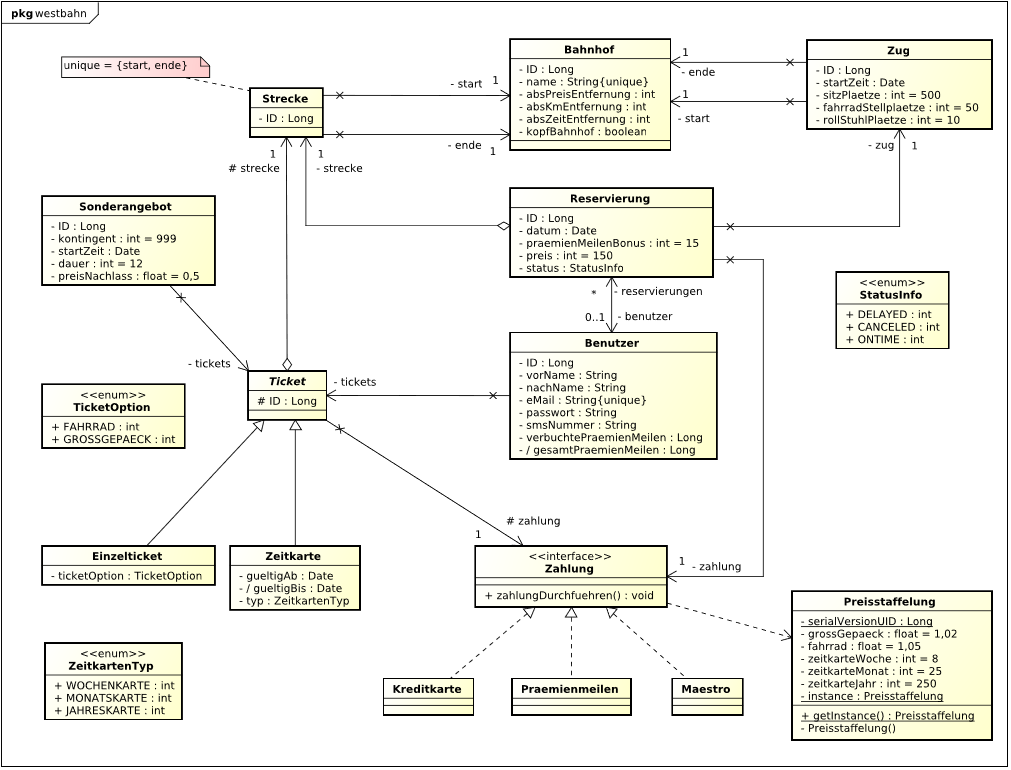
\includegraphics[width=1\linewidth]{images/uml}
	\caption{UML}
	\label{fig:uml}
\end{figure}

\clearpage

Erstellen Sie von folgendem Modell Persistenzklassen und implementieren Sie diese mittels JPA:\\

Westbahn Domänenmodell\\

Suche
Die Suche nach Zügen muss auf jeden Fall die Auswahl des Abfahrts- und Ankunftsortes (nur folgende Bahnhöfe sind möglich: Wien Westbhf, Wien Hütteldorf, St. Pölten, Amstetten, Linz, Wels, Attnang-Puchheim, Salzburg) ermöglichen. Dies führt zur Anzeige der möglichen Abfahrten, die zur Vereinfachung an jedem Tag zur selben Zeit stattfinden. Des weiteren wird auch die Dauer der Fahrt angezeigt.\\

In dieser Liste kann nun eine gewünschte Abfahrtszeit ausgewählt werden. Die Auswahl der Zeit führt zu einer automatischen Weiterleitung zum Ticketshop.\\

Um sich die Auslastung der reservierten Sitzplätze anzusehen, muss bei dem Suchlisting noch das Datum ausgewählt werden. Dieses Service steht jedoch nur registrierten Benutzern zur Verfügung.\\

Ticketshop
Man kann Einzeltickets kaufen, Reservierungen für bestimmte Züge durchführen und Zeitkarten erwerben. Dabei sind folgende Angaben notwendig:\\

Einzeltickets: Strecke (Abfahrt/Ankunft), Anzahl der Tickets, Optionen (Fahrrad, Großgepäck)
Reservierung: Strecke (Abfahrt/Ankunft), Art der Reservierung (Sitzplatz, Fahrrad, Rollstuhlstellplatz), Reisetag und Zug (Datum/Uhrzeit)\\
Zeitkarte: Strecke, Zeitraum (Wochen- und Monatskarte)\\

Um einen Überblick zu erhalten, kann der Warenkorb beliebig befüllt und jederzeit angezeigt werden. Es sind keine Änderungen erlaubt, jedoch können einzelne Posten wieder gelöscht werden.\\

Die Funktion „Zur Kassa gehen“ soll die Bezahlung und den Ausdruck der Tickets sowie die Zusendung per eMail/SMS ermöglichen. Dabei ist für die Bezahlung nur ein Schein-Service zu verwenden um zum Beispiel eine Kreditkarten- bzw. Maestrotransaktion zu simulieren.\\

Prämienmeilen
Benutzer können sich am System registrieren um getätigte Käufe und Reservierungen einzusehen. Diese führen nämlich zu Prämienmeilen, die weitere Vergünstigungen ermöglichen. Um diese beim nächsten Einkauf nützen zu können, muss sich der Benutzer einloggen und wird beim „Zur Kassa gehen“ gefragt, ob er die Prämienmeilen für diesen Kauf einlösen möchte.\\

Instant Notification System der Warteliste
Der Kunde soll über Änderungen bezüglich seiner Reservierung (Verspätung bzw. Stornierung) mittels ausgesuchtem Service (eMail bzw. SMS) benachrichtigt werden. Bei ausgelasteten Zügen soll auch die Möglichkeit einer Anfrage an reservierte Plätze möglich sein. Dabei kann ein Zuggast um einen Platz ansuchen, bei entsprechender Änderung einer schon getätigten Reservierung wird der ansuchende Kunde informiert und es wird automatisch seine Reservierung angenommen.\\

\clearpage

Sonderangebote
Für festzulegende Fahrtstrecken soll es ermöglicht werden, dass ein fixes Kontingent von Tickets (z.b.: 999) zu einem verbilligten Preis (z.b.: 50\% Reduktion) angeboten wird. Diese Angebote haben neben dem Kontingent auch eine zeitliche Beschränkung. Der Start wird mit Datum und Uhrzeit festgelegt. Die Dauer wird in Stunden angegeben. Diese Angebote werden automatisch durch Ablauf der Dauer beendet.\\

Task 1 - Mapping
Schreiben Sie für alle oben definierten Klassen und Relationen entsprechende Hibernate JPA Implementierungen (javax.persistence.*). Bis auf die Klasse Reservierung sollen dafür die Annotationen verwendet werden. Die Klasse Reservierung soll mittels XML Mapping definiert werden.\\

Task 2 - Named Queries
Schreiben Sie folgende NamedQueries (kein plain SQL und auch keine Inline-Queries) für das Domänenmodell aus Task1. Die Queries sollen die entsprechenden Parameter akzeptieren und die gewünschten Typen zurückliefern:\\

a) Finde alle Reservierungen für einen bestimmten Benutzer, der durch die eMail-Adresse definiert wird.\\
b) Liste alle Benutzer auf, die eine Monatskarte besitzen.\\
\\

Task 3 - Validierung
Alle Constraints der einzelnen Entitäten sollen verifiziert werden. Hierfür soll die Bean Validation API verwendet werden. Folgende Einschränkungen sollen überprüft werden:

a) Zug und Strecke können nicht denselben Start- und Endbahnhof besitzen.\\
b) Die eMail des Benutzers soll ein gängiges eMail-Pattern befolgen.\\
c) Die Startzeit eines Sonderangebotes kann nicht in der Vergangenheit liegen.\\
d) Der Name eines Bahnhofs darf nicht kürzer als zwei und nicht länger als 150 Zeichen sein. Sonderzeichen sind bis auf den Bindestrich zu unterbinden.\\


\subsection{Bewertung} 

Gruppengrösse: 1 Person\\
Anforderungen "überwiegend erfüllt"\\
Dokumentation und Beschreibung der angewendeten Schnittstelle\\
Task 1\\
Task 2\\
Anforderungen "zur Gänze erfüllt"
Task 3\\
Ausreichende Testobjekte zur Validierung der Persistierung
Überprüfung der funktionalen Anforderungen mittels Regressionstests

\clearpage

\section{Abgabe} 
Es ist ein Protokoll (TGM-HIT/latex-protocol) sowie der Link zum Github-Repository (als Kommentar) hier abzugeben. Die Durchführung der Übung ist mittels regelmäßigen Commits zu dokumentieren. Zum Abgabegespräch ist das Protokoll ausgedruckt vorzulegen (doppelseitig, beidseitig - an langer Kante).

\section{Quellen} 

''The Java EE Tutorial - Persistence''; Oracle; online: https://docs.oracle.com/javaee/7/tutorial/partpersist.htm\#BNBPY\\
''HTML5 - A vocabulary and associated APIs for HTML and XHTML"; W3C; 17.12.2012; online: https://www.w3.org/TR/2012/CR-html5-20121217/forms.html\#valid-e-mail-address\\
"Hibernate ORM Documentation"; JBoss; online: http://hibernate.org/orm/documentation/5.2/l\\
"JPA Westbahn"; Maven Project structure; online: https://github.com/TGM-HIT/syt4-jpa-westbahn\\
''Hibernate ORM 5.2.13 Final User Guide''; JBoss; 25.01.2018; online:\\ https://docs.jboss.org/hibernate/orm/5.2/userguide/html\_single/Hibernate\_User\_Guide.html 	% Information about the purpose of this project
\section{Umsetzung}

\subsection{Entities}

Aus dem UML Diagramm wurden Java Klassen generiert. Zu diesen wurden die Notwendigen Annotationen hinzugefügt. 

\subsubsection{Annotationen}

	Hibernate bietet zur Konfiguration der Entities Annotationen an. 
	
	\begin{itemize}
		\item[] @Entity: wird verwendet um Klassen als Entitäten zu markieren
		\item[] @Id: legt Attribute als Primary Key fest
		\item[] @GeneratedValue: erstellt automatisch ID Werte
		\item[] @Column: kann besondere eigenschaften für die Tabellenspalte festlegen
		\subitem name: legt den Namen fest
		\subitem unique: stellt sicher, dass dieser Wert eindeutig ist
		\item[] @Transient: speichert Attribute nicht in der Datenbank
		\item[] @OneToOne: eindeutige Beziehung zwischen Enitäten
		\item[] @OneToMany: legt fest das eine Collection von einer Enität zu mehreren anderen ist
		\item[] @ManyToOne: legt fest das mehrere Entitäten eine Beziehun zu einer Enität haben
		\item[] @ManyToMany: erstellt Beziehungen zwischen Collections von Entitäten und mehreren Entitäten
		\subitem cascade: Legt fest wie die Beziehungen behandelt werden sollen
		  
	\end{itemize}

	\begin{code}[]{java}
	public class Benutzer {
		
		@Id
		@GeneratedValue(strategy = GenerationType.AUTO)
		private Long ID;
		
		@NotNull
		private String vorName;
		
		@NotNull
		@CorrectEmailConstraint
		private String eMail;
		
		@NotNull
		private String passwort;
		
		@OneToMany(cascade = CascadeType.ALL)
		private Set<Ticket> tickets;
		
		@OneToMany(cascade = CascadeType.ALL)
		private Set<Reservierung> reservierungen;
	}
	\end{code}

	\clearpage

	\subsection{XML-Mapping}
	
	Bis auf die Klasse ''Reservierung'' wurden alle mit Annotationen erstellt. ''Reservierung'' wurde mit XML-Mapping erstellt. Dies bietet die Möglichkeit unabhängig von der Klassendatei das Mapping festzulegen. Weiters ist es sinnvoll, wenn es schon eine bestehende Datenbankstruktur gibt.
	
	Das Mapping für die Klasse ''xyz'' muss in der Datei ''xyz.hbm.xml'' festgelegt werden.
	
	\begin{itemize}
		\item[] <hibernate-mapping>: Erstellt ein neues Hibernate mapping
		\item[] <class>: Legt fest für welche Klasse das Mapping gilt
		\subitem name: Name bzw. Ort der Klasse. Z.b. entity.Reservierung
		\subitem table: Legt den Name der Datenbanktabelle fest
		\subitem <id: Legt Primärschlüssel fest
		\subsubitem name: Name des Attributs
		\subsubitem <generator>: Legt die Art der Generierung fest
		\subitem <property>: Legt das Mapping für ein Attribut fest
		\subsubitem name: Name des Attributs
		\subsubitem column: Spaltenname
		\subsubitem type: Klassenname oder Ort
		\subitem <many-to-one>: So wie property, nur für Many to One. Syntax gilt auch für alle anderen Kardinalitäten.
	\end{itemize}
	
	\begin{code}[]{java}
		<?xml version = "1.0" encoding = "utf-8"?>
		<!DOCTYPE hibernate-mapping PUBLIC
		"-//Hibernate/Hibernate Mapping DTD//EN"
		"http://www.hibernate.org/dtd/hibernate-mapping-3.0.dtd">
		
		<hibernate-mapping>
		<class name = "entity.Reservierung" table = "Reservierung">
		
		<meta attribute = "class-description">
		Sis is a reserwayschion.
		</meta>
		
		<id name = "ID" type = "java.lang.Long" column = "id">
		<generator class="identity"/>
		</id>
		
		<property name = "datum" column = "datum" type = "java.util.Date"/>
		<property name = "praemienMeilenBonus" column = "praemienMeilenBonus" type = "int"/>
		<property name = "preis" column = "preis" type = "int"/>
		<property name = "status" column = "status" type = "entity.StatusInfo"/>
		<many-to-one cascade="all" name = "benutzer" class = "entity.Benutzer"/>
		<many-to-one cascade="all" name = "strecke"  class = "entity.Strecke"/>
		<many-to-one cascade="all" name = "zug" class = "entity.Zug"/>
		
		</class>
		</hibernate-mapping>
	\end{code}
	
	\section{Setup}
	
	Das Projekt wurde mit Maven umgesetz.
	
	\subsection{Maven}
	
	Für Maven wurden folgende Abhängigkeiten in  ''pom.xml'' definitert.
	
	\begin{itemize}
		\item org.hibernate:hibernate-core:5.3.1.Final
		\item com.h2database:h2:1.4.197
		\item org.hibernate.validator:hibernate-validator:6.0.10.Final
		\item org.apache.maven.plugins:maven-surefire-plugin:2.21.0
		\item junit:junit:4.12
		\item org.glassfish:javax.el:3.0.1-b08
	\end{itemize}

	\subsection{Hibernate}
	
	Für Hibernate wurde ein ''hibernate.cfg.xml'' erstellt. 
	
	\subsubsection{H2}
	
	Damit Hibernate mit der H2 Datenbank kommunizieren kann wurde folgendes Konfiguriert:
	
	\begin{code}[]{java}
		<hibernate-configuration>
		<session-factory>
		<property name="hibernate.connection.driver_class">org.h2.Driver</property>
		<property name="connection.url">jdbc:h2:mem:test</property>
		<property name="connection.username">sa</property>
		<property name="connection.password"/>
		<property name="hibernate.dialect">org.hibernate.dialect.H2Dialect</property>
	\end{code}
	
	\subsubsection{Entitäten}
	
	Damit die Entitäten von Hibernate erkannt werden wurde folgendes Konfiguriert:
	
	\begin{code}[]{java}
		<mapping class="entity.Bahnhof"/>
		<mapping class="entity.Benutzer"/>
		<mapping class="entity.Einzelticket"/>
		<mapping class="entity.Reservierung"/>
		<mapping class="entity.Strecke"/>
		<mapping class="entity.Zeitkarte"/>
		<mapping class="entity.Zug"/>
		<mapping class="entity.Sonderangebot"/>
		
		<mapping resource="Reservierung.hbm.xml" />
	\end{code}

	\section{Hibernate}
	\subsection{Session}
	Um ein Sessionobjekt zu erstellen, wurd eine Sessionfactory erstellt.
	
	\begin{code}[]{java}
		return new Configuration().configure("hibernate.cfg.xml").buildSessionFactory();
	\end{code}

	\subsection{Persistierung}
	Damit ein Objekt persistiert werden kann muss eine Transaktion erstellt werden. In dieser kann dann die Funktion ''persist'' aufgerufen werden, um eine Entität zu Speichern. 
	Damit nicht alle Attribute, welche Entitäten sind, einzeln Persistiert werden müssen wurde zu allen ''cascade = CascadeType.ALL'' hinzugefügt.
	
	\begin{code}[]{java}
		session = HibernateUtil.getSessionFactory().openSession();
		
		for(int i = 0; i < 20;++i) {
			session.beginTransaction();
			Benutzer b = FakeDataGenerator.generateRandomBenutzer();
			b = FakeDataGenerator.addReservationsToBenutzer(b);
			benutzers.add(b);
			
			session.persist(b);
			session.getTransaction().commit();
		}
	\end{code}


	\subsection{Validierung}
	
	Mittels Validierungsannotationen können Attribute oder Klassen auf korrektheit überprüft werden.
	
	\begin{itemize}
		\item @NotNull: Attribut darf nicht ''null'' sein
		\item @Email: Validiert eine Email pattern
		\item @Pattern: Regex überprüfung von Strings
		\item @Past: Datum muss in der Vergangenheit liegen
		\item @Future: Datum miss in der Zukunft liegen
		\item @FutureOrPresent/@PastOrPresent
	\end{itemize}
	
	\clearpage
	
	\subsection{Named Queries}
	
	\subsubsection{Syntax von HQL}
	
	\begin{itemize} 
		\item SELECT: ''SELECT''
		\item Spalten: ''spaltenname'' 
		\item AS: ''Benutzer ben'' legt eine Kurzbezeichnung für die Klasse fest
		\item Subqueries: Sind in ''IN'' möglich
		\item Where: Gleich wie in SQL
		\item Parameter: '':varname'' kennzeichnet einen Parameter
	\end{itemize}
	
	\subsection{Definition}
	Die Named-Queries können entweder in ''hibernamte.cfg.xml'' festgelegt werden, order mit Annotationen.
	
	\begin{code}[]{java}
		@NamedQueries({
			@NamedQuery(
			name = "ReservationsViaEmail",
			query = "SELECT reservierungen FROM entity.Benutzer b WHERE b.eMail = :email"
			)
		)
	\end{code}
	
	\subsubsection{Aufgaben queries}
	
	\begin{enumerate}
		\item SELECT reservierungen FROM entity.Benutzer b WHERE b.eMail = :email
		\item SELECT DISTINCT b From entity.Benutzer b, entity.Zeitkarte z WHERE z.typ = entity.ZeitkartenTyp.MONATSKARTE AND b.tickets.ID = z.ID
		\item SELECT t FROM entity.Ticket t INNER JOIN t.strecke s where s not in (select strecke FROM entity.Reservierung)
	\end{enumerate}
	
	\subsubsection{Aufrufen}
		Named-queries können mittels der Session abgefragt und ausgeführt werden.
	\begin{code}[]{java}
		List<Reservierung> reservierungs = session.getNamedQuery("ReservationsViaEmail").setParameter("email",a.geteMail()).list();
		
		Iterator<Reservierung> it = a.getReservierungen().iterator();	
	\end{code}

	\clearpage

\section{Probleme}
	
	 % Solution for the given tasks and their documentation
% \glsaddall 		% Add all glossary entries to printglossaries
\end{document}
